\documentclass[french,12pt,a4paper]{report}


\usepackage[utf8]{inputenc}
\usepackage[T1]{fontenc}
\usepackage{babel}
\usepackage[top=3cm, bottom=3cm, left=2cm, right=2cm]{geometry}
\usepackage{graphics}
\usepackage{graphicx}
\usepackage{eurosym}
\usepackage{soul}
\usepackage{graphicx} %utilisation d'images
\usepackage{amsmath}
\usepackage{relsize}
\usepackage{titlepic}
\usepackage{times}
\usepackage{url}
\usepackage{listings}
\usepackage[]{algorithm2e}
\usepackage{hyperref}
\usepackage{amsfonts}
\usepackage{dsfont}

\begin{titlepage}
\newcommand*{\defeq}{\stackrel{\mathsmaller{\mathsf{def}}}{=}}
\title{Résumé de BaddEtAl16}
\author{DUGUE Clément}
\date{\today}
\end{titlepage}



\begin{document}

\hypersetup{linkcolor=blue}
\maketitle
\tableofcontents


\chapter{Introduction}

\section{Répartition des Points}


%%%%%%%%%%%%%%%%%%%%%%%%%%%%%%%%%%%%%%%%%%%%%%%%%%%%%%%%%%%%%%%%
\subsection{Les Points}
%\indent
Lorsqu'on rassemble des données pour une étude (localisation d'évènements, d'objets, de populations...), il peut être utile de représenter ces données sous forme de points. On obtient alors une répartition ponctuelle des données pouvant alors être analysée. On peut ainsi identifier des tendances selon la densité des points (si les points sont rapprochés ou non), c'est l'analyse statistique. Enfin les résultats de l'analyse peuvent être interprétés pour en tirer des conclusions.\\

L'analyse statistique d'une répartition de points est utile pour de nombreux domaines. En effet, elle permet de repérer objectivement des informations graphiques que l'on n'aurait pas pu distinguer à l'oeil nu. De plus une répartition spatial de point est souvent un substitut à des variables innobservables physiquement (exposition à la pollution, événements historiques).\\

Cependant, il n'y a pas de solution toute faite pour l'analyse statistique de répartition de points. En effet chaque cas doit être analysé en fonction de son contexte (obtention des données, objectif de l'analyse).\\


%%%%%%%%%%%%%%%%%%%%%%%%%%%%%%%%%%%%%%%%%%%%%%%%%%%%%%%%%%%%%%%%
\subsection{Les points de differents types}

\begin{minipage}[c]{0.45\linewidth}
 Les points d'une représentation peuvent être classés en différents types. L'analyse de la distribution portera alors sur une comparaison des positions et densités des points de chaque type.\\
 
La figure 1.1.2 montre par exemple la répartition de bouleaux et de chênes dans une foret. Une analyse pertinente serait de regarder si les 2 types d'arbres ont la même distribution spatiale ou si la proportion relative des 2 espèces varie sur le domaine.
\end{minipage}
\hfill
\begin{minipage}[c]{0.45\linewidth}
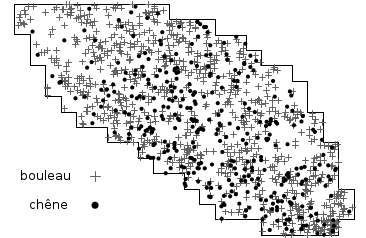
\includegraphics[scale=0.6]{images/diffPoints.png}\\
\small{FIGURE 1.1.2 - Exemple de répartition ponctuelle de 2 types d'arbres dans un forêt}
\end{minipage}

%%%%%%%%%%%%%%%%%%%%%%%%%%%%%%%%%%%%%%%%%%%%%%%%%%%%%%%%%%%%%%%%
\subsection{Répartition de point marqués}
\begin{minipage}{0.45\linewidth}
Marquer un point permet d'ajouter une information auxiliaire sur ce point (taille d'un arbre, masse d'une étoile).\\

La figure 1.1.3 montre par exemple la répartition d'arbre d'une forêt, et chaque arbre est représenté par un cercle plus ou moins gros en fonction de son diamètre en cm. On peut alors analyser la répartition des arbres en fonction de leur diamètre.
\end{minipage}\hfill
\begin{minipage}{0.45\linewidth}
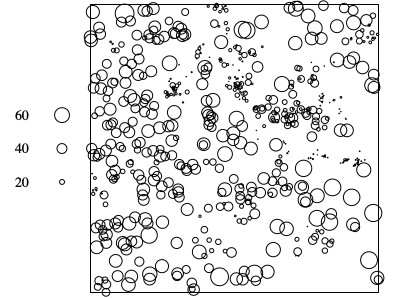
\includegraphics[scale=0.5]{images/pointsMarques.png}\\
\small{FIGURE 1.1.3 - Exemple de répartition ponctuelle des diamètres des arbres d'une forêt}
\end{minipage}

%%%%%%%%%%%%%%%%%%%%%%%%%%%%%%%%%%%%%%%%%%%%%%%%%%%%%%%%%%%%%%%%
\subsection{Covariables}
Les bases de données peuvent aussi inclure des covariables: des variables pouvant donner une explication sur le résultat de l'étude. Ces données ne répondent pas à une question statistiques, elles sont utilisées pour expliquer le phénomène mis en évidence par l'étude.\\

\begin{minipage}{0.45\linewidth}
La figure 1.1.4 montre par exemple la répartition des arbres d'une forêt, avec une information d'altitude donnée en fond. Le but de l'étude est de connaitre la répartition de densité des arbres de la forêt. Ici l'information sur l'altitude est une covariable car elle propose une explication possible du résultat de l'analyse de densité: les arbres poussent mieux à une altitude modérée.
\end{minipage}\hfill
\begin{minipage}{0.45\linewidth}
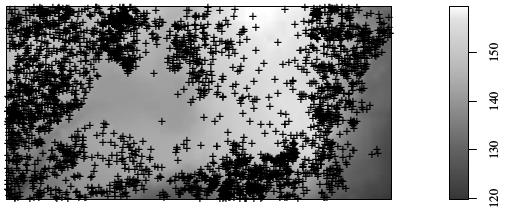
\includegraphics[scale=0.5]{images/covariables.png}\\
\small{FIGURE 1.1.4 - Exemple de répartition ponctuelle d'abre d'une forêt avec information sur l'altitude}
\end{minipage}
\\

%%%%%%%%%%%%%%%%%%%%%%%%%%%%%%%%%%%%%%%%%%%%%%%%%%%%%%%%%%%%%%%%
\subsection{Differentes dimensions spatiales}
Les localisations des points son généralement en 2 dimensions, mais on peut tout autant avoir une représentation spatiale en 1 dimension (accidents sur un réseau routier), en 3 dimensions (observation de cellules par un microscope 3D), ou même en espace-temps (localisation spatiale et temporel des épicentres de tremblement de terre). Ainsi l'analyse de répartition spatiale de points n'est pas réservée à un nombre de dimension particulier, on pourrait imaginer le faire pour n-dimensions.\\


%%%%%%%%%%%%%%%%%%%%%%%%%%%%%%%%%%%%%%%%%%%%%%%%%%%%%%%%%%%%%%%%
\subsection{Reproduction de répartitions}
On peut comparer des données prises à des données récoltés à des moment et endroits different pour en faire une analyse, c'est la reproduction d'expérience.\\
Cette reproduction fournit des données pouvant être analysées indépendemment. Mais on peut aussi croiser ces nouvelles informations avec les données précédemment analysées pour minimiser des facteurs extérieurs.\\
Par exemple, une répartition de population dans une ville peut être très dense autour d'un stade s'il y a un événement sportif dans la ville. Ainsi la répétition de l'expérience sur plusieurs semaines permettra, en prenant la moyenne des résultats, d'avoir une analyse non biaisée par l'événement.\\

%%%%%%%%%%%%%%%%%%%%%%%%%%%%%%%%%%%%%%%%%%%%%%%%%%%%%%%%%%%%%%%

\section{Méthodes statistiques pour l'analyse de répartition de point}

\subsection{Statistiques sommaires}
L'approche traditionnelle pour analyser une répartition de point est de calculer une statistique sommaire qui est censée capturer une caractéristique importante de la répartition ponctuelle. Par exemple connaître la distance du plus proche voisin moyenne pour une répartiton d'arbre dans une forêt. Une statistique sommaire peut être pratique si elle est utilisée de façon simple et appropriée, afin que ses valeurs puissent être facilement interprétés.\\
Cependant en réduisant une répartition spatiale de point à une simple information, on perd beaucoup d'information. On peut avoir un même résultat pour des répartitons spatiales de point totalement differentes. Trouver une expliquation n'est alors pas simple, on ne peut pas forcement en tirer de conclusion.

\subsection{Modèle statistique et inférence}
Les statistiques sommaire marchent bien pour des situations simples. Pour des situations plus complexes, il est plus commode d'utiliser un modèle statistique. C'est une description d'un essemble de données décrivant les moyennes, tendance et relations systématiques entre les données, mais aussi la variabilité de la donnée. Par exemple lorsqu'on trace une ligne sur un nuage de point, un modèle regressif nous donne la position de la ligne mais également le regroupement des points autour de cette ligne. On peut ainsi générer de nouveaux nuages de points ayant les mêmes propriétés.

\subsection{Validation}

La préocupation principale lors d'une modélisation est de savoir si le modèle peut être faux. Les techniques pour valider le modèle permettent de savoir si le modèle est plutôt bon dans l'ensemble, de critiquer chaque supposition du modèle, de comprendre les faiblesses de l'analyse et de détecter les anomalies.\\

\begin{minipage}[c]{0.45\linewidth}
La figure 1.2.3 montre par exemple l'influence de chaque donnée: plus un point modifie le modèle si on l'enlève plus sa représentation est grosse sur la figure. Ainsi le diamètre des cercles est proportinnel à l'influence des points sur le modèle. On voit une influence disproportionnée en bas à gauche de l'image, ainsi soit les données de ce coin sont des anomalies, soit le modèle n'est pas approprié.
\end{minipage}
\hfill
\begin{minipage}[c]{0.45\linewidth}
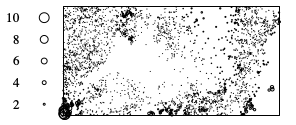
\includegraphics[scale=0.8]{images/validation.png}\\
\small{FIGURE 1.2.3 - Influence de chaque point sur le modèle}
\end{minipage}

%%%%%%%%%%%%%%%%%%%%%%%%%%%%%%%%%%%%%%%%%%%%%%%%%%%%%%%%%%%%%%%%
%%%%%%%%%%%%%%%%%%%%%%%%%%%%%%%%%%%%%%%%%%%%%%%%%%%%%%%%%%%%%%%%

\chapter{Correlation (chap. 7)}

\section{Introduction}

Le but de l'analyse d'une répartition de données ponctuelles est en général de déterminer si la position d'un point est indépendante ou non de celle d'un autre. Il y a alors 3 formes typiques de représentations:
\begin{itemize}
\item répulsif (les points ont tous une certaine distance les uns des autres);
\item aléatoire (les points n'ont pas de dépendance);
\item agrégée (les points forment des groupes de points).\\
\end{itemize}

\begin{center} 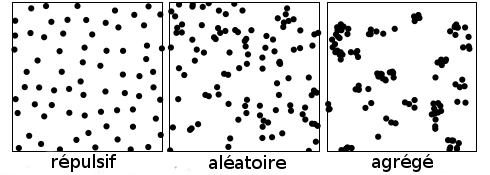
\includegraphics[scale=0.8]{images/repartition.png} \end{center}

Un outil standard pour mesurer cette dépendance est la covariance (moment d'ordre 2). La variance d'une variable aléatoire permet de quantifier les variations d’une variable par rapport à sa moyenne (moment d'ordre 1). La covariance va alors permettre de quantifier les variations simultanées de deux variables aléatoires par rapport à leur moyenne respective.
Les avantages de la covariance sont qu'elle est facile à calculer et à manipuler. Ses inconvénients sont qu'elle requière une bonne estimation de la moyenne  et ne permet pas de determiner la cause des regroupements de point (car c'est une statistique sommaire).
Il faut alors trouver d'autre fonctions pour analyser les dépendances de position des points.\\
%%%%%%%%%%%%

\section{L'indice de Ripley : fonction K}

\subsection{La fonction K empirique}
Supposons qu'on se pose une question sur l'espacement entre les points dans un ensemble de points. Il serait alors naturel de mesurer la distance \begin{math} d_{ij} = ||x_i-x_j||\end{math} entre chaque point distinct \begin{math} x_i \end{math} et \begin{math} x_j \end{math} de l'ensemble \textbf{X} considéré. Si ces distances sont grandes, la répartition de point serait plutôt répulsive. Alors que si elles sont petites, la répartition de point serait plutôt aggrégée.\\

Considérons alors la fonction de distribution cumulative empirique des distances par paires:
\begin{align*}
\hat{H}(r) &= \text{taux des valeurs } d_{ij} \text{ plus petites que r } \\
        &= \frac{1}{n(n-1)} \sum_{i=1}^n \sum_{\underset{j \neq i}{j=1}}^n \mathds{1} \{d_{ij} \leq r \}
\end{align*}
défini pour chaque distance \begin{math} r \geq 0 \end{math}. La fonction indicatrice  \begin{math} \mathds{1} \{...\}\end{math} vaut 1 si son contenu est vrai et 0 sinon. La somme de ces indicatrices est simplement le nombre de fois où le contenu est vrai: le nombre de distance entre chaque point inférieur ou égal à r. Le déniominateur n(n-1) est le nombre total des paires de points distincts.\\

\begin{minipage}[c]{0.45\linewidth}
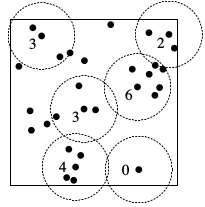
\includegraphics[scale=0.9]{images/nombreVoisins.png}\\
\small{FIGURE 2.2.1 - Nombre de points voisin dans un certain rayon}
\end{minipage}
\hfill
\begin{minipage}[c]{0.45\linewidth}
Comme le montre la figure 2.2.1, on cherche à estimer le nombre moyen de voisin dans un certain rayon r sur une certaine surface. Ainsi pour standardiser l'équation, il faut diviser l'expression par l'intensité \begin{math}\lambda \end{math} et pas seulement par (n-1). On peut alors approximer l'intensité sur la surface telle que: \begin{math}\lambda = (n-1)/|W|\end{math} où |W| est l'aire de la surface étudiée.\begin{math}|W|\end{math}. Les points où le rayon dépassent du bord de la surface ne donneront pas des résultats exactes, il ne faut donc pas non plus négliger les effets de bords.
\end{minipage}\\

La fonction \begin{math}|W|\hat{H}(r)\end{math} est la moyenne standardisée du nombre de points voisins dans un rayon r pour un point type. Afin de prendre en compte les effets de bords, on ajoute une correction pour les effets de bords à \begin{math}\hat{H}\end{math}, ce qui nous donne la fonction K empirique:
\begin{align*}
\hat{K}(r) = \frac{|W|}{n(n-1)} \sum_{i=1}^n \sum_{\underset{j \neq i}{j=1}}^n \mathds{1} \{d_{ij} \leq r \} e_{ij}(r)
\end{align*}
où \begin{math}e_{ij}(r)\end{math} est une correction pour les effets de bords qui sera expliquée plus loin.\\

%%%%%%%%%%%%

\subsection{La vraie fonction K pour un processus de points}

\begin{minipage}{0.45\linewidth}
La fonction empirique \begin{math}\hat{K}(r)\end{math} est un relevé des distances des paires de points dans la répartition de points. Mais pour connaître les informations que nous donne cette cette fonction il faut la comparer avec la vraie fonction K théorique pour un processus de Poisson homogène. C'est à dire qu'il faut connaître la fonction K dans le cas d'une répartition des point totalement aléatoire. Cette fonction qu'on appellera \begin{math}K_{pois}(r)\end{math} est donnée par la surface couverte par r:
\begin{center}\begin{math} K_{pois}(r) = \pi r^2 \end{math}\end{center}
La figure 2.2.2 montre alors la représentation en fonction de r de la fonction K théorique.
\end{minipage}\hfill
\begin{minipage}{0.45\linewidth}
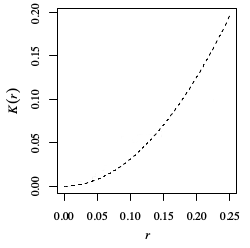
\includegraphics[scale=0.9]{images/Kpoiss.png}
\small{FIGURE 2.2.2 - Représentation de la fonction K pour une répartition totalement aléatoire}
\end{minipage}

%%%%%%%%%%%%

\subsection{Inteprétation de K}
La figure ci dessous montre la fonction estimé de K selon si la répartition est agrégée aléatoire ou bien répulsif. Les traits discontinues sont la représentation graphique de la fonction K théorique pour un aléatoire total.\\

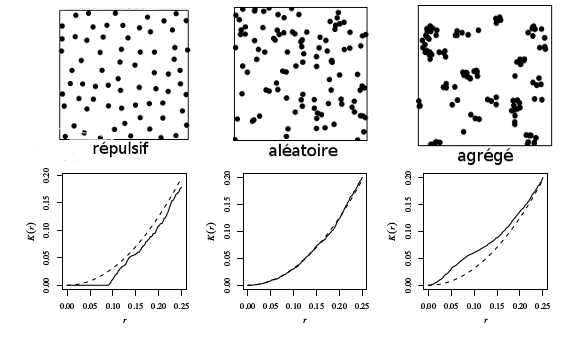
\includegraphics[scale=0.7]{images/interpret3.png}

Sur la gauche, la courbe de la fonction calculée est en dessous de celle pour une répartition totalement aléatoire (\begin{math}\hat{K}(r) < K_{pois}(r) \end{math}). Ainsi, pour une distance r, un point quelconque a en moyenne moins de voisins qu'il aurait pu espérer avoir avec une répartition totalement aléatoire. Donc la répartition est répulsive.\\
\indent
Sur la droite, la courbe de la fonction calculée est au dessus de celle pour une répartition totalement aléatoire (\begin{math}\hat{K}(r) > K_{pois}(r) \end{math}). Ainsi, pour une distance r, un point quelconque a en moyenne plus de voisins qu'il aurait pu espérer avoir avec une répartition totalement aléatoire. Donc la répartition est agrégée.\\

%%%%%%%%%%%%

\section{Correction des bords}


Une stratégie simple pour corriger les problèmes d'estimation sur les bords est la méthode de restriction des bords. Lorsqu'on fait une estimation de K(r) pour une distance r, on limite les calculs aux point se trouvant à une distance r du bord de la surface étudiée. Ainsi le cercle de rayon r autour du point loge entièrement dans la surface comme le montre la figure 2.3.

\begin{center}
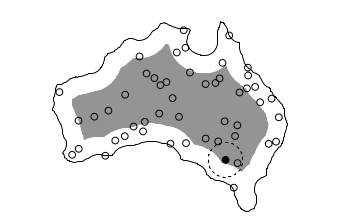
\includegraphics[scale=0.7]{images/bords.png}\\
\small{FIGURE 2.2.3 -Exemple de zone de sureté pour un certain rayon}\\
\end{center}

Ainsi en prenant en compte que les points dans la zone de sureté pour chaque r, on peut réécrire \begin{math} \hat{K}(r) \end{math}. Ainsi en gardant les même notation qu'au 2.2.1, on a peut écrire la fonction K avec correction des bords \begin{math} \hat{K}_{bord}(r) \end{math} telle que:
\begin{align*}
\hat{K}_{bord}(r) = \frac{  \sum_{i=1}^n \mathds{1} \{b_i \geq r \} \sum_{\underset{j \neq i}{j=1}}^n \mathds{1} \{d_{ij} \leq r \}}{\lambda \sum_{i=1}^n \mathds{1} \{b_i \geq r \}}
\end{align*}
où \begin{math}b_i\end{math} est la distance d'un point \begin{math}x_i\end{math} au bord de la surface, et \begin{math}\lambda\end{math} est l'estimation de l'intensité soit \begin{math}\lambda = n/|W|\end{math} avec |W| aire de la surface.

%%%%%%%%%%%%%%%%%%%%%%%%%%%%%%%%%%%%%%%%%%%%%%%%%%%%%%%%%%%%%%%%
%%%%%%%%%%%%%%%%%%%%%%%%%%%%%%%%%%%%%%%%%%%%%%%%%%%%%%%%%%%%%%%%

\chapter{Espacement (chap. 8)}

\section{Introduction}
Les fonctions statistiques, telle que la fonction K, mesurant la corrélation spatiale dans un processus de point sont des outils très populaire pour évaluer la dépendance. Cependant avec cette méthode, certains aspects de la dépendance ne peuvent être observés. Il faut alors utiliser des mesures sur les espaces vides ou bien sur les plus petites distances entre les points.

%%%%%%%%%%%%%%%%

\section{Fonction d'espace vide F}

\subsection{Définitions pour un processus de point stationnaire}
Si X est un processus de point spatial, la distance:
\begin{center}\begin{math} d(u,X) = min\{ ||u-x_i|| : x_i \in X \} \end{math}\end{center}
d'une position \begin{math} u \in \mathbb{R} \end{math} au plus proche point d'un processus est appelé 'distance d'espace vide'.\\
Pour un processus de point stationnaire, la fonction de distance d'espace vide est:
\begin{center}\begin{math} F(r) = \mathbb{P}\{ d(u,X) \leq r \} \end{math}\end{center}
définie pour toute distance \begin{math} r \geq 0 \end{math}, où u est une position quelconque.\\

Les valeurs de F(r) sont les probabilités (entre 0 et 1) pour n'importe quel point u, qu'il y ait un point X présent dans à une distance r ou moins de u (qu'il y ait un point dans le cercle de rayon r autour de u).\\

%%%%%%%%%%%%%%%%

\subsection{Valeurs pour un aléatoire complet}

\begin{minipage}{0.45\linewidth}
Pour un aléatoire complet, la fonction F suit une fonction de répartition de Poisson uniforme sur la surface d'un cercle (\begin{math} \pi r^2 \end{math}) soit pour une intensité \begin{math} \lambda \end{math} : 
\begin{center}\begin{math} F_{pois}(r) = 1 - exp(-\lambda \pi r^2) \end{math}\end{center}
C'est la fonction d'espace vide F théorique pour un aléatoire total.\\
La figure 3.2.2 montre la représentation en fonction de r de cette fonction théorique.
\end{minipage}\hfill
\begin{minipage}{0.45\linewidth}
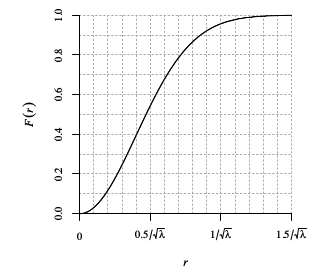
\includegraphics[scale=0.7]{images/poisson.png}
\small{FIGURE 3.2.2 - Représentation de la fonction de répartition de Poisson}
\end{minipage}

%%%%%%%%%%%%%%%%

\subsection{Estimation discrète de F}
"à faire"
Montrer la somme avec explication et la correction d'effets de bords

%%%%%%%%%%%%%%%%

\subsection{Interprétation de F}
La figure ci dessous montre la fonction estimé de F selon si la répartition est agrégée aléatoire ou bien répulsif. Les traits discontinues sont la représentation graphique de la fonction F théorique pour un aléatoire total.\\

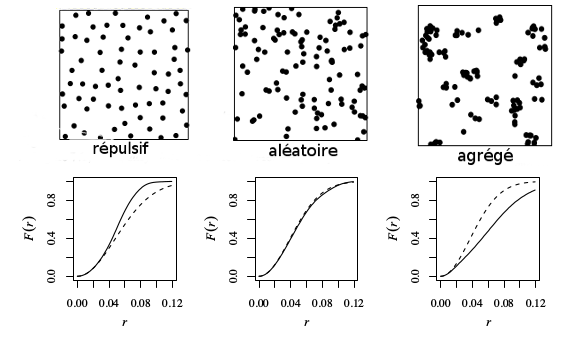
\includegraphics[scale=0.7]{images/interpret.png}

Sur la gauche, la courbe de la fonction calculée est au dessus de celle pour une répartition totalement aléatoire (\begin{math}\hat{F}(r) > F_{pois}(r) \end{math}). Ainsi, pour une distance r, la probabilité que \begin{math} d(u,X) \leq r \end{math} est plus grande quelle ne l'est pour une répartition aléatoire, les espaces vides sont donc plus petits que prévu. Donc la répartition est répulsive.\\
\indent
Sur la droite, la courbe de la fonction calculée est en dessous de celle pour une répartition totalement aléatoire (\begin{math}\hat{F}(r) < F_{pois}(r) \end{math}). Ainsi, pour une distance r, la probabilité que \begin{math} d(u,X) \leq r \end{math} est plus petite quelle ne l'est pour une répartition aléatoire, les espaces vides sont donc plus grands que prévu. Donc la répartition est agrégée.



%%%%%%%%%%%%%%%%%%%%%%%%%%%%%%%%%%%%%%%%%%%%%%%%%%%%%%%%%%%%%%%

\section{Fonction de plus proche voisins G}

\subsection{Définitions pour un processus de point stationnaire}
Si \begin{math}x_i\end{math} est un des points d'une représentation de points \textbf{x}, la distance du plus proche voisin de  \begin{math}x_i\end{math} est écrite telle que:
\begin{center}\begin{math} d_i = d(x_i,\textbf{x}\backslash x_i ) \end{math}\end{center}
la plus courte distance de \begin{math} x_i \end{math} à un autre point de \textbf{x} excepté \begin{math} x_i \end{math}.
Pour un processus de point stationnaire X, la fonction de distance du plus proche voisin est:
\begin{center}\begin{math} G(r) = \mathbb{P}\{ d(u,X\backslash u) \leq r | u \in X\} \end{math}\end{center}
définie pour toute distance \begin{math} r \geq 0 \end{math}, où u est une position quelconque.\\

%%%%%%%%%%%%%%%%

\subsection{Valeurs pour un aléatoire complet}

Pour un aléatoire complet, la fonction G est égale à la fonction d'espace vide F. Soit pour un un processus homogène de Poisson: 
\begin{center}\begin{math} G_{pois}(r) = 1 - exp(-\lambda \pi r^2) \end{math}\end{center}
Celà n'est vrai que pour une répartition totalement aléatoire, en général F et G seront des fonctions différentes.\\

%%%%%%%%%%%%%%%%

\subsection{Estimation discrète de G}
"à faire"
Montrer la somme avec explication et la correction d'effets de bords

%%%%%%%%%%%%%%%%

\subsection{Interprétation de G }
La figure ci-dessous montre la fonction estimée de G selon si la répartition est agrégée aléatoire ou bien répulsif. Les traits discontinus sont la représentation graphique de la fonction G théorique pour un aléatoire total.\\

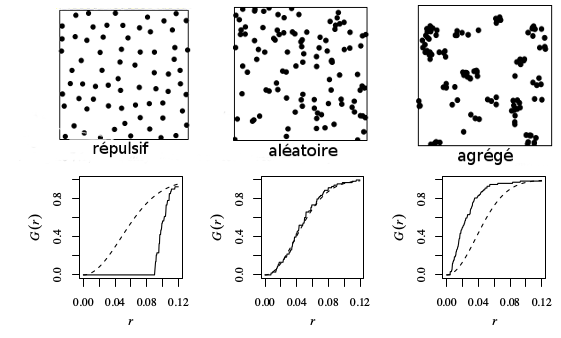
\includegraphics[scale=0.7]{images/interpret2.png}

Sur la gauche, la courbe de la fonction calculée est en dessous de celle pour une répartition totalement aléatoire (\begin{math}\hat{G}(r) < G_{pois}(r) \end{math}). Ainsi, les distances des plus proches voisins sont plus grandes que celles prévues pour une répartiton aléatoire. Donc la répartion est répulsive.\\
\indent
Sur la droite, la courbe de la fonction calculée est au dessus de celle pour une répartition totalement aléatoire (\begin{math}\hat{G}(r) > G_{pois}(r) \end{math}). Ainsi, les distances des plus proches voisins sont plus petites que celles prévues pour une répartiton aléatoire. Donc la répartion est agrégée.\\


%%%%%%%%%%%%%%%%
\section{Fonction J}

Les distances du plus proche voisin et les distances d'espace-vide ont la même distribution de probabilité si la répartition des point est totalement aléatoire. Pour les départs des expériences avec une répartission aléatoire complète, ces distances ont tendance à répondre dans des directions opposées: l'un devient plus grand et l'autre plus petit. Cela suggère qu'une comparaison de ces 2 types de distance pourrait être utile pour évaluer les départs d'une répartition aléatoire.\\

Une combinaison pratique de G et F, suggérée par la théorie fondamentale, est la fonction J d'un processus stationnaire ponctuel:
\begin{center}\begin{math} J(r) = \frac{1-G(r)}{1-F(r)} \end{math}\end{center}
définie pour tout \begin{math} r \geq 0 \end{math} telle que F(r) < 1. Pour un processus de Poisson homogène, \begin{math} F_{pois} \equiv G_{pois} \end{math} ainsi les valeures de J(r) > 1 son cohérent avec une représentation répulsive, tandis que les valeures de J(r) < 1 sont cohérente avec une représentation agrégée.

La fonction J empirique est insensible aux effets de bords, car ceux-ci s'annulent dans le ratio (1 - G)/(1 - F).

%%%%%%%%%%%%%%%%

\end{document}
